\documentclass[a4paper, 12pt]{report}
\usepackage[french]{babel}
\usepackage[utf8]{inputenc}
\usepackage[T1]{fontenc}
\usepackage{lmodern}
\usepackage{amsmath}
\usepackage{amsfonts}
\usepackage{hyperref}
\usepackage{listings}
\usepackage[top=3cm, bottom=3cm, left=2.5cm, right=2.5cm]{geometry}
\usepackage{graphicx}
\usepackage{setspace}
\usepackage{fancyhdr}
\usepackage{titlesec}
\usepackage{xcolor}

\usepackage{forest}

\lstset{
  basicstyle=\ttfamily\small,
  keywordstyle=\color{blue},
  commentstyle=\color{gray},
  stringstyle=\color{red},
  breaklines=true,
  numbers=left,
  numberstyle=\tiny,
  frame=single
}


\newcommand{\HRule}{\rule{\linewidth}{0.5mm}}

\begin{document}
\lefthyphenmin=62
\righthyphenmin=62

\begin{titlepage}
	\begin{center}
		\textsc{\LARGE Institut National des Sciences Appliquées de Rouen}
		\vspace{5mm}
		\bigbreak
		
\includegraphics[width=0.48\textwidth]{logo.png}\\[1.0 cm]
		\textsc{\Large ITI3}\\[0.5cm]
		\textsc{\Large Projet Intégratif Développement Orienté Objet}\\
		\vspace{0.2cm}
		% Title
		\hspace{1pt}
		\setstretch{1,8}
		\HRule \\[1pt]
		{\huge \bfseries Développement orienté objet
		du projet ITI Aventure}\\[0.4cm]
		\HRule \\[0.5cm]
		\singlespacing    
		% Author and supervisor
		\begin{minipage}{0.4\textwidth}
			\begin{flushleft} \large
				\emph{Auteurs:}\\
				Mohamed Aziz \textsc{Ayari} \\
				{\small\href{mailto:maya00@insa-rouen.fr}{maya00@insa-rouen.fr}}\\
				Joachim \textsc{Curtelin}\\
				{\small\href{mailto:joachim.curtelin@insa-rouen.fr}{joachim.curtelin@insa-rouen.fr}}
				\\
				Hamza \textsc{Fadili} \\
				{\small\href{mailto:hamza.fadili@insa-rouen.fr}{hamza.fadili@insa-rouen.fr}}
				\\
				Louis \textsc{Lenoble} \\
				{\small\href{mailto:louis.lenoble@insa-rouen.fr}{louis.lenoble@insa-rouen.fr}}
				\\
				Jack \textsc{Su} \\
				{\small\href{mailto:jack.su@insa-rouen.fr}{jack.su@insa-rouen.fr}}
				\\
			\end{flushleft}
		\end{minipage}
		\begin{minipage}{0.4\textwidth}
			\begin{flushright} \large
				\emph{Enseignants:} \\
				Robin \textsc{Condat} \\
				{\small\href{mailto:robin.condat@insa-rouen.fr}{robin.condat@insa-rouen.fr}}
				\\
				Nicolas \textsc{Delestre} \\
				{\small\href{mailto:nicolas.delestre@insa-rouen.fr}{nicolas.delestre@insa-rouen.fr}}
				\\
        		Géraldine \textsc{Del Mondo} \\
				{\small\href{mailto:geraldine.del\_mondo@insa-rouen.fr}{geraldine.del\_mondo@insa-rouen.fr}}
				\\
				Nicolas \textsc{Malandain} \\
				{\small\href{mailto:nicolas.malandain@insa-rouen.fr}{nicolas.malandain@insa-rouen.fr}}
				\\
				Laurent \textsc{Vercouter} \\
				{\small\href{mailto:laurent.vercouter@insa-rouen.fr}{laurent.vercouter@insa-rouen.fr}}
				\\
			\end{flushright}
		\end{minipage}
		\vfill
		{\large \today}
	\end{center}
\end{titlepage}

\begingroup
\titleformat{\part}[display]
    {\normalfont \bfseries\centering}{}{0pt}{\Huge}
\titleclass{\part}{straight}
\titlespacing*{\part}{0pt}{50pt}{90pt}
\endgroup

\begingroup
\titleformat{\chapter}[display]
    {\normalfont \bfseries\centering}{}{0pt}{\Huge}
\titleclass{\chapter}{straight}
\titlespacing*{\chapter}{0pt}{50pt}{90pt}
\addtocontents{toc}{\vspace{-0.7cm}}
\endgroup

\titlespacing*{\subsection}
    {30pt}{9pt}{6pt}

\newpage

\tableofcontents

\newpage

\chapter{Introduction}

Dans le cadre de notre troisième année à l’INSA Rouen Normandie, nous avons été amenés à participer aux Projets Intégratifs (PI). 
Ces projets ont pour objectif principal de nous permettre de mettre en pratique l’ensemble des compétences acquises tout au long de notre cursus.

Le projet sur lequel nous avons travaillé vise à assurer la bonne persistance du jeu \textit{ITI Aventure}, et s’articule autour de trois axes principaux :
Tout d’abord, nous avons mis en place une solution permettant de sauvegarder et de charger une partie depuis une base de données (BD).
Ensuite, nous avons conçu un interpréteur capable de charger une partie à partir d’un fichier structuré.
Enfin, nous avons modifié l’architecture du projet afin d’intégrer le design pattern \textit{Factory}, dans le but de généraliser et de simplifier la création de différents types d’aventures.



\chapter{Persistance BD}

Dans cette partie, notre objectif est d’établir un lien entre la logique métier du jeu et une base de données, 
afin de pouvoir sauvegarder l’état d’une partie. Pour ce faire, nous devons mettre en place un système de mapping objet-relationnel, permettant de 
faire correspondre les objets du jeu aux données stockées dans la base.

Nous utilisons le langage Java, qui propose l’API JDBC (Java Database Connectivity). 
Cette API permet à une application Java de se connecter à une base de données, d’exécuter des requêtes SQL, 
et de traiter les résultats de manière structurée.

\section{Description et fonctionnement}
\subsection{Passage du modèle entité-association en modèle relationnel}

La première étape consiste à établir un modèle entité-association. Celui-ci nous a été founit au début du projet. Nous devons donc le transformer en modèle relationnel. Pour cela, nous nous sommes du cours de BD1 à notre disposition.

\begin{figure}[h]
    \centering
	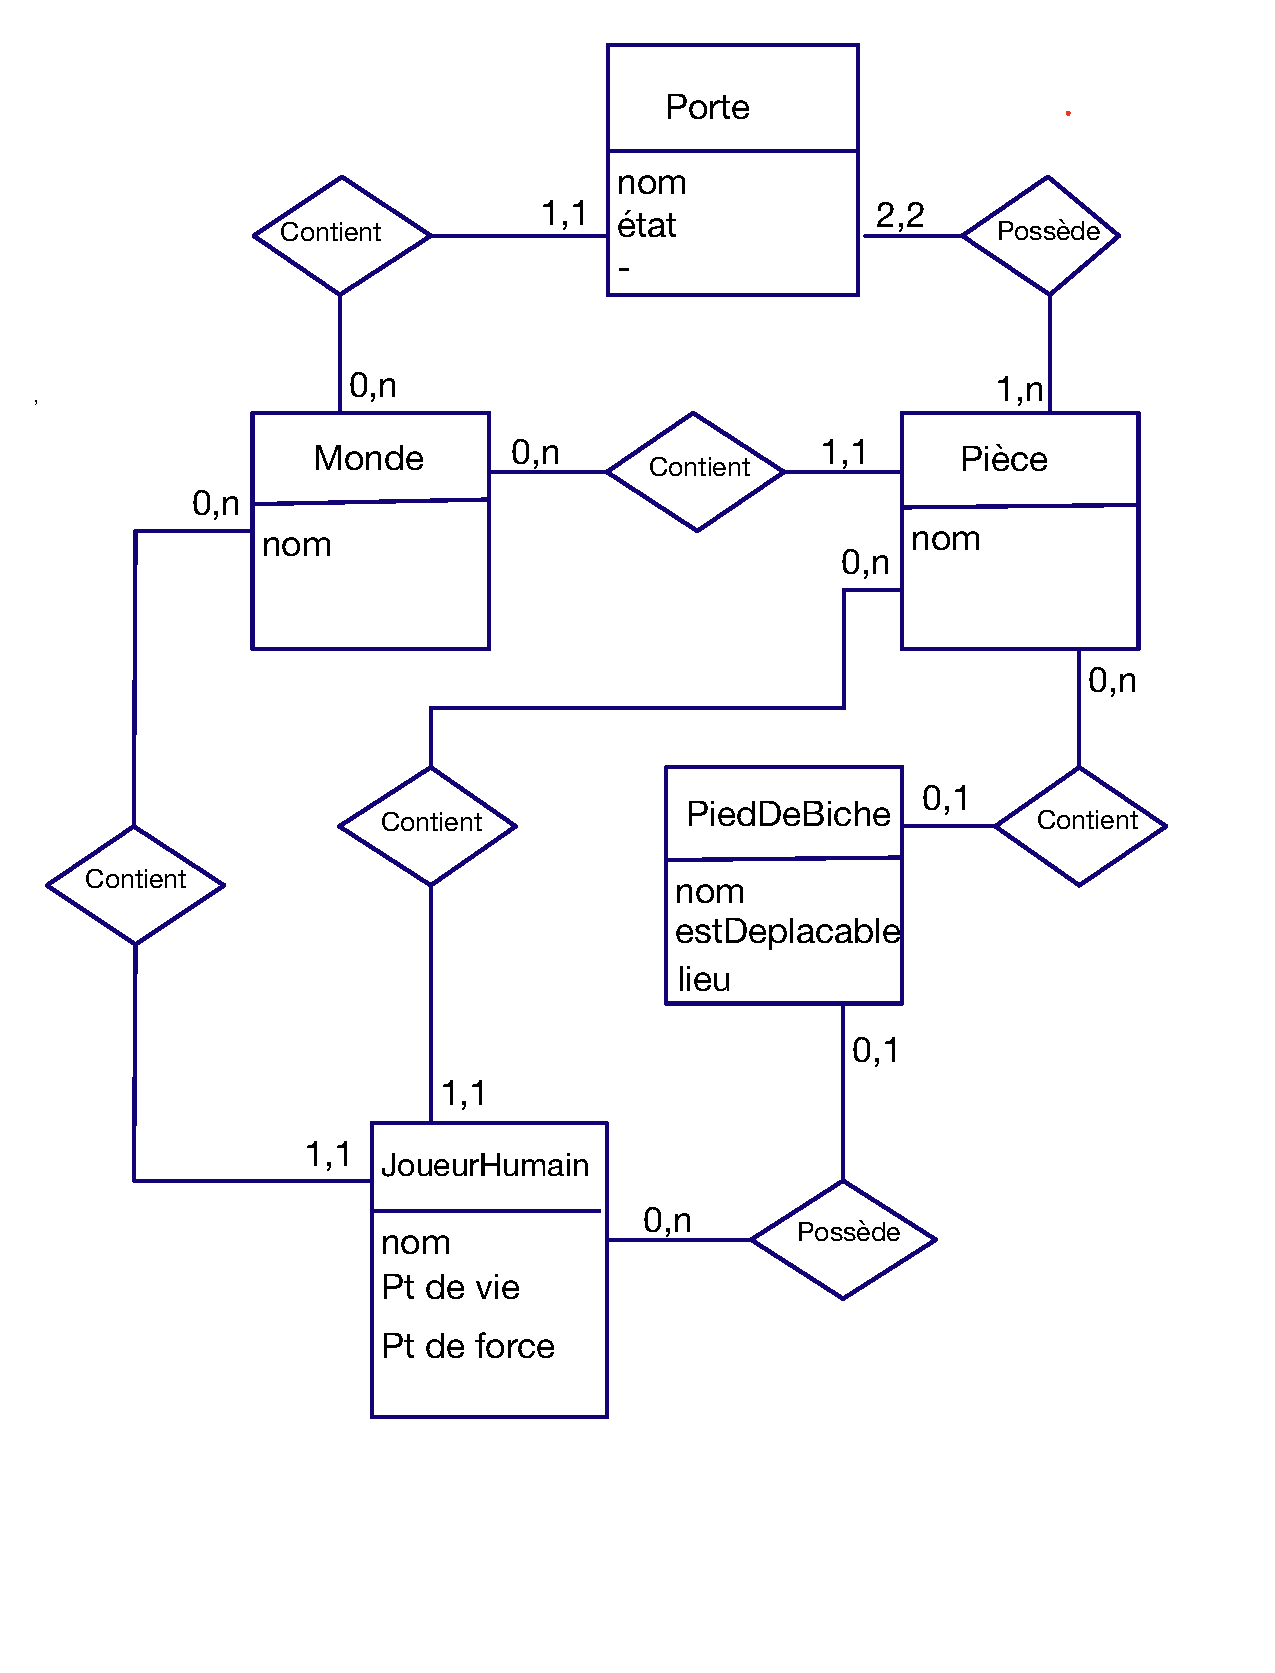
\includegraphics[width=0.35\textwidth]{BD-EA.pdf}
    \caption{Schéma entités-associations pour ITI Aventure}
\end{figure}

Explication des transformations:\\
\begin{enumerate}
    \item Cas 1 : Entités en relation : Les objets qui rentrent dans le cas 1.
    \begin{itemize}
	    \item Monde d'attribut nom en MONDE(nom)
	    \item Porte d'attributs nom et état en PORTE(nom,etat)
	    \item PiedDeBiche d'attributs nom, estDéplaceable en PIEDEBICHE(nom,estDéplaceable)
	    \item JoueurHumain d'attributs nom, pV, pF, en JOUEURHUMAIN(nom, pV, pF)
	    \item Pièce d'attribut nom en PIECE(nom)
    \end{itemize}
    \item Cas 2 : Entités faibles en relations.
    Il n y'a pas d'entités faibles dans notre table EA.
    \item Cas 3 : Association binaire 1-1 par clés étrangères. Les entités concernées sont les suivantes : 
    \begin{itemize}
           \item PORTE reçoit la clé de Monde comme attribut qui est nomMonde.
           \item JOUEURHUMAIN la clé de Monde et la clé de PIECE comme attributs qui sont nomMonde et nomPiece.
           \item PIECE reçoit la clé de Monde comme attribut qui est nomMonde.
     \end{itemize}
     \item Cas 4 : Association binaire M-N. Les entités concernées sont les suivantes :
     \begin{itemize}
     	\item PIECEPOSSEDEPORTE reçoit les clés de PORTE et PIECE comme clés, qui sont nomPiece et nomPorte. Il aurait été possible de transformer cette relation par le cas 3 : association binaire 2-2, en associant dans la table PORTE deux attributs, pieceA et pieceB.
     	\item PIECECONTIENTPDB reçoit comme clés, les clés de PIECE et PIEDDEBICHE et qui sont nomPiece et nomPiedDeBiche.
     	\item JOUEURPOSSEDEPDB reçoit comme clés, les clés de JOUEURHUMAIN et PIEDDEBICHE, qui sont nomJoueur et nomPiedDeBiche.
     \end{itemize}
    
\end{enumerate}
\vspace{1cm}
Voici le résultat final:
\begin{itemize}
    \item \textbf{MONDE}(\underline{nom})
    \item \textbf{PORTE}(\underline{nom}, etat, nom\_monde)
    \item \textbf{PIEDDEBICHE}(\underline{nom}, estDeplaceable)
    \item \textbf{JOUEURHUMAIN}(\underline{nom}, ptVie, ptForce, nom\_monde, nom\_piece)
    \item \textbf{PIECE}(\underline{nom}, nom\_monde)
    \item \textbf{JOUEURPOSSEDEPDB}(\underline{nom\_joueur}, \underline{nom\_pied\_de\_biche})
    \item \textbf{PIECECONTIENTPDB}(\underline{nom\_piece}, \underline{nom\_pied\_de\_biche})
    \item \textbf{PIECEPOSSEDEPORTE}(\underline{nom\_porte}, \underline{nom\_piece})\\
\end{itemize}


Maintenant que nous avons définit notre modèle relationnel, nous pouvons commencer à travailler avec nos tables SQL. 
Pour cela, nous initialisation les tables vides grâce à un fichier Initialisation.sql. Ensuite, nous avons développé la classe LecteurBD qui implémente l'interface 
Lecteur de notre projet ITI Aventure. Cette dernière s'occupe de lire chaque table (en envoyant une instruction SQL via un PreparedStatement) de chaque relation et de créer 
ou assigner les attributs de chaque objet. Nous avons procédé de la même manière pour la classe EnregistreurBD.
Cette classe s'occupe de vider les tables à chaque instanciation, puis de récupérer chaque objet du monde et de les enregistrer dans la table correspondante. 

\subsection{EnregistreurBD}
La classe EnregistreurBD a été utilisée pour sauvegarder l’état du jeu. Dans notre contexte, elle a permis d’enregistrer le monde du jeu, les pièces, 
les portes qui relient deux pièces, ainsi que les objets et entités tels que le joueur humain ou le pied-de-biche. Cette classe joue le rôle de pont entre 
les objets Java et la base de données, assurant la persistance des données. Elle utilise JDBC pour interagir avec la base et permet de traduire l’état du jeu en requêtes SQL.

Les étapes de l'enregistrement sont les suivantes:

\begin{itemize}
\item établir une connexion à la base de données.
\item préparer la requête à l'aide de PrepareStatement (l'insertion dans notre cas).

\item utiliser comme des méthodes comme setString ou setInt pour attribuer aux paramètres de la requête les valeurs des attributs à enregistrer (par exemple, le nom d'une pièce ou les points de force).

\item exécuter pour insérer ou mettre à jour les données dans la base (executeUpdate).

\item fermer la requête.

\item fermer la connexion à la base de données.

\end{itemize}

Ces étapes sont répétées pour chaque entité du jeu (sauf la fermeture de connexion avec la BD), tout en respectant l’ordre d’enregistrement imposé par les dépendances entre les tables. (voir Annexe~\ref{annexe:exemple-enregistrement})

\subsection{LecteurBD}

La classe LecteurBD est utilisée pour lire les données depuis la base de données. Elle permet de charger l'état du jeu précédemment enregistré, en reconstruisant les différentes entités et leurs relations. Cette classe joue un rôle essentiel de mapping entre les données persistées dans la base et les objets Java.

Les étapes du chargement sont les suivantes (voir Annexe~\ref{annexe:exemple-lecture}): 

\begin{itemize}
  \item Se connecter à la base de données.
  
  \item Préparer la requête de recherche avec une instruction SELECT.
  
  \item Exécuter la requête et récupérer les résultats dans un ResultSet.
  
  \item Parcourir chaque ligne du ResultSet à l'aide de la méthode next().
  
  \item Récupérer les valeurs des colonnes avec des méthodes comme
getString() ou getInt().

  \item Instancier les objets correspondants à partir des données récupérées.
  
  \item Fermer la requête.
    
  \item Fermer la connexion à la base de données.
\end{itemize}

\chapter{Interprétation fichier structuré}
\section{Lecture du format du fichier structuré}

Dans ce projet, une manière de charger des données du jeu est d'interpréter un fichier structuré avec un langage fonctionnel.
C'est pourquoi dans cette partie, nous verrons comment nous avons fait pour décomposer ce type de fichier
afin de l'implémenter dans notre jeu ITIAventure. Un fichier \texttt{exemple.cfg} nous est donné (voir Annexe~\ref{annexe:exemple-cfg})

La structure du fichier se présente ainsi :
\begin{itemize}
	\item Le fichier présenté est un fichier de configuration
	\item Chaque ligne de ce fichier de configuration est une affectation
	\item L'affectation fera appel à une fonction dont le retour sera stockée dans une variable
	\item Les paramètres de ces appels de fonction pourront être des identifiants, des constantes ou des appels de fonction
	\item Tout identifiant devra être affecté, et donc déclaré, avant d'être utilisé
	\item Les constantes pourront être:
	\begin{itemize}
		\item \texttt{SUCCES, ECHEC, ENCOURS}
		\item Des chaînes de caractères entourés de doubles guillemets
		\item Des nombres entiers
	\end{itemize}
\end{itemize}

Afin d'exploiter notre fichier de configuration, il est nécessaire d'avoir un outil qui permet d'interpréter ce langage.
C'est pourquoi nous utilisons \texttt{JavaCC} (Java Compiler Compiler) qui permet de créer automatiquement un analyseur lexical et un analyseur syntaxique.

\section{Écriture de la grammaire}

À partir du fichier de configuration et des règles sur la structure du fichier, nous pouvons écrire la grammaire suivante (avec les unités lexicales) :

\begin{flushleft}
	\begin{tabbing}
		\hspace{4.2cm} \= \kill % indentation
		$\langle \text{CONFIGURATION} \rangle$ \> ::= $\text{AFFECTATION}$+ \\
		$\langle \text{AFFECTATION} \rangle$ \> ::= ID AFF $\text{APPEL\_FONCTION}$ \\
		$\langle \text{APPEL\_FONCTION} \rangle$ \> ::= IDF PARAG $\text{PARAMS}$ PARAD \\
		$\langle \text{ID} \rangle$ \> ::= [A-Z,a-z,\_][A-Z,a-z,0-9,\_]$\ast$ \\
		$\langle \text{AFF} \rangle$ \> ::= "=" \\
		$\langle \text{VIR} \rangle$ \> ::= "," \\
		$\langle \text{IDF} \rangle$ \> ::= "monde" | "piece" | "serrure" | "porte" | "pied\_de\_biche" | "cle" | \\ "monstre" | "humain" |
		"cdf\_vivant\_dans\_piece" | "cdf\_vivant\_possede" | "cdf\_conjonction" \\
		$\langle \text{PARAG} \rangle$ \> ::= "(" \\
		$\langle \text{PARAD} \rangle$ \> ::= ")" \\
		$\langle \text{PARAMS} \rangle$ \> ::= $\text{PARAM}$ ($\text{VIR}$ $\text{PARAM}$)$\ast$ \\
		$\langle \text{PARAM} \rangle$ \> ::= ID \ | \ CHAINE \ | \ NB\_ENTIER \ | \ $\text{APPEL\_FONCTION}$ | CONST \\
		$\langle \text{CONST} \rangle$ \> ::= "SUCCES" \ | \ "ECHEC" \ | \ "ENCOURS" \\
		$\langle \text{CHAINE} \rangle$ \> ::= \texttt{'"'}$\text{LETTRE}$+\texttt{'"'} \\
		$\langle \text{LETTRE} \rangle$ \> ::= caractère alphanumérique \\
		$\langle \text{NB\_ENTIER} \rangle$ \> ::= [0-9]+
	\end{tabbing}
\end{flushleft}

\noindent
Explication de la grammaire :
\begin{itemize}
	\item \textbf{$\langle \text{CONFIGURATION} \rangle$}~: une configuration est composée d'une ou plusieurs affectations.
	\item \textbf{$\langle \text{AFFECTATION} \rangle$}~: une affectation associe un identifiant à un appel de fonction, séparés par un signe égal.
	\item \textbf{$\langle \text{APPEL\_FONCTION} \rangle$}~: un appel de fonction commence par un identifiant de fonction, suivi d'une parenthèse ouvrante, d'une liste de paramètres, puis d'une parenthèse fermante.
	\item \textbf{$\langle \text{ID} \rangle$}~: un identifiant commence par une lettre ou un underscore, suivi de zéro ou une infinité de lettres, chiffres ou underscores.
	\item \textbf{$\langle \text{AFF} \rangle$}~: le symbole d'affectation est le signe égal \texttt{=}.
	\item \textbf{$\langle \text{VIR} \rangle$}~: les paramètres sont séparés par des virgules.
	\item \textbf{$\langle \text{IDF} \rangle$}~: les identifiants de fonction sont des mots-clés prédéfinis correspondant aux entités du jeu.
	\item \textbf{$\langle \text{PARAG} \rangle$} et \textbf{$\langle \text{PARAD} \rangle$}~: parenthèses ouvrante et fermante pour entourer les paramètres d'une fonction.
	\item \textbf{$\langle \text{PARAMS} \rangle$}~: une liste de paramètres, séparés par des virgules.
	\item \textbf{$\langle \text{PARAM} \rangle$}~: un paramètre peut être un identifiant, une chaîne, un nombre entier, un appel de fonction (imbriqué dans une fonction), ou une constante.
	\item \textbf{$\langle \text{CONST} \rangle$}~: une constante est l'un des mots \texttt{SUCCES}, \texttt{ECHEC} ou \texttt{ENCOURS}.
	\item \textbf{$\langle \text{CHAINE} \rangle$}~: une chaîne de caractères est entourée de guillemets et contient une ou plusieurs lettres.
	\item \textbf{$\langle \text{LETTRE} \rangle$}~: une lettre est un caractère alphanumérique.
	\item \textbf{$\langle \text{NB\_ENTIER} \rangle$}~: un nombre entier est composé d'un ou plusieurs chiffres.
\end{itemize}

\section{Lecture de l'AST}

Après l'analyse syntaxique du fichier de configuration, un Arbre Syntaxique Abstrait (AST) est généré automatiquement à partir de la grammaire définie dans \texttt{AnalyseurSyntaxique.jj}. 
Cet AST représente la structure du fichier, où chaque n\oe ud correspond à une unité lexicale du langage.

\begin{figure}[htbp]
	\centering
	\begin{forest}
		for tree={
			draw,
			ellipse,
			font=\sffamily,
			align=center,
			edge={-latex, thick},
			parent anchor=south,
			child anchor=north
		}
		[Configuration
			[Affectation
				[ID]
				[AppelFonction
					[IDF]
					[Paramètres
						[Paramètre
							[AppelFonction]
							[Chaine]
							[Constante]
							[ID]
							[NbEntier]
						]
					]
				]
			]
		]
	\end{forest}
	\caption{Représentation de l'Arbre Syntaxique Abstrait}
\end{figure}


Pour exploiter cet AST, nous avons implémenté le patron de conception \texttt{Visiteur} ainsi que l'interface \texttt{Visitable}. 

Chaque classe représentant un n\oe ud de l'AST implémente l'interface \texttt{Visitable}, qui définit une méthode \texttt{accepter}. Le visiteur contient alors une méthode \texttt{visiter} spécifique pour chaque type de n\oe ud. 

Ainsi, lors de la lecture de l'AST, il suffit de parcourir l'arbre en appelant la méthode \texttt{visiter} sur la racine, et le visiteur se charge de traiter chaque nœud selon sa nature.

Dans notre cas, notre classe qui implémente \texttt{Visiteur} sera un lecteur de jeu, nommé \texttt{LecteurAST.java}.
Cette classe prendra comme paramètre dans son constructeur un fichier de configuration. 
Il ira visiter l'AST généré à partir de ce fichier, en parcourant chaque n\oe ud. Ce lecteur joue alors un rôle d’analyseur sémantique et intervient dans la phase de traitement, en vérifiant et en instanciant les entités du jeu.

\section{Relation entre variable et entité du jeu}

Un problème rencontré dans l'implémentation du \texttt{LecteurAST.java} a été la gestion des variables déclarées et leurs entités dans le jeu.

En effet, lors de la lecture du fichier de configuration, chaque affectation crée une nouvelle entité du jeu (par exemple une pièce, une porte, une clé, etc.) et l'associe à un identifiant (variable). Pour assurer ce lien, nous avons utilisé une structure de type \texttt{HashMap<String, String>} appelée \texttt{tableDesNoms}, qui fait le lien entre chaque identifiant déclaré et le nom de l'entité correspondante.

Lors du parcours de l'AST, la méthode \texttt{visiter(Affectation aff)} extrait l'identifiant de l'affectation ainsi que le nom de l'entité (lorsqu'il s'agit d'une chaîne de caractères parmi les paramètres de l'appel de fonction). Si ce nom est trouvé, il est nettoyé de ses guillemets éventuels puis ajouté à la table de correspondance. Ainsi, à chaque nouvelle affectation, le couple identifiant-nom est enregistré dans la table. Cela permet, lors de l'utilisation ultérieure d'un identifiant comme paramètre dans un autre appel de fonction, de retrouver rapidement le nom associé à cet identifiant.


\chapter{Design Patterns}
Le but de cette dernière partie est de modifier l'architecture du projet ITI Aventure afin de généraliser et simplifier la création d'une aventure. 
\section{Description et fonctionnement}
Pour être indépendant du type des classes, nous avons implémenté le design pattern "Abstract Factory" de la facon suivante : ITIAventureFactory est la factory depuis laquelle les autres héritent. 
Ensuite, Monde, Monstre, Pièce, Porte, Serrure, Clé sont non seulement des produits et mais aussi les produits desquels tous les autres produits héritent. 
La classe LecteurDescription utilise ainsi l'une ou l'autre Factory pour instancier les objets en fonction de la première ligne du fichier de description.

Pour mieux comprendre, voici le diagramme UML représentant l'utilisation de ce design pattern:

\begin{figure}[h]
	\centering
	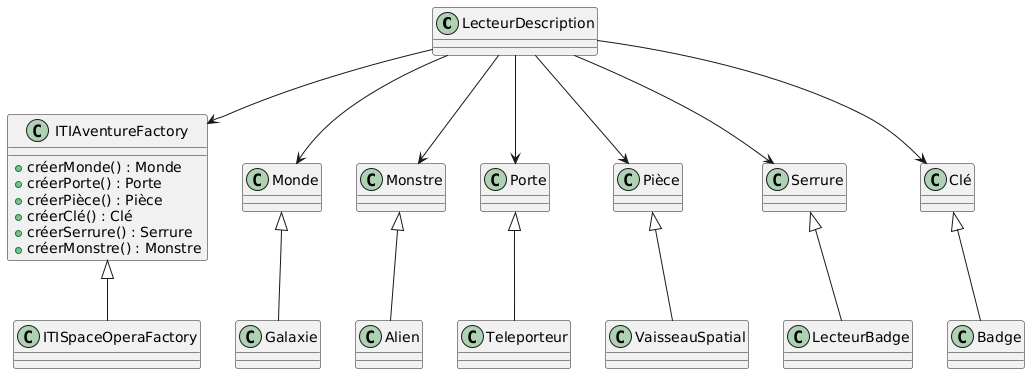
\includegraphics[width=1\textwidth]{DP.png}\\[1.0 cm]
	\caption{Diagramme UML du design pattern factory pour ITI Aventure}
\end{figure}
On constate que pour créer une nouvelle aventure, il suffit simplement de développer une nouvelle classe (comme ITISpaceOperaFactory), chargée d’instancier les objets spécifiques, eux-mêmes hérités des éléments d’une aventure standard.

\chapter*{Conclusion générale}

Ce projet nous a permis de mettre en pratique de nombreuses compétences acquises durant notre formation, en particulier autour du développement orienté objet, de la persistance des données et de la conception logicielle. 
Nous avons appris à manipuler une base de données relationnelle, à écrire un interpréteur avec JavaCC, à générer et parcourir un AST, et à structurer notre code avec des design patterns comme Factory ou Visiteur.

Grâce à ce travail, nous avons conçu une architecture claire, modulaire et facilement extensible, ce qui facilite l'ajout de nouveaux types d'aventures ou de nouvelles entités de jeu.

Pour aller plus loin, nous pourrions réfléchir à implémenter une interface Homme-Machine afin de rendre le jeu plus intuitif, ou encore à développer un outil rendant la création de fichiers de configuration plus facile.
Nous pourrions alors nous aider de la bibliothèque graphique JavaSwing qui a été abordé en cours.

\bigbreak
\begin{figure}[htbp]
	\centering
	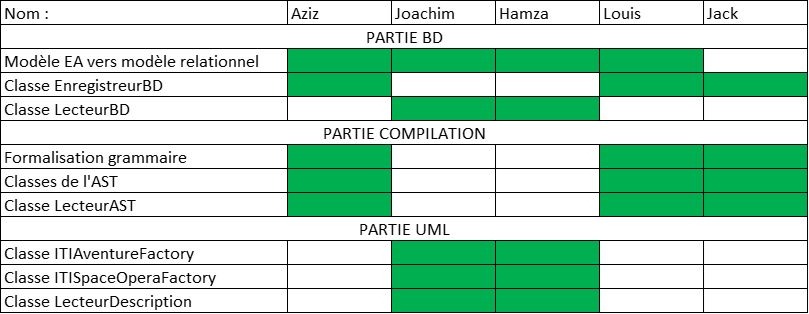
\includegraphics[width=1\textwidth]{matrice_repartition.png}\\[1.0 cm]
	\caption{Matrice de répartition du projet}
\end{figure}

\appendix
\chapter{Annexes BD}
\section{Annexe : Exemple de code d'enregistrement}
\label{annexe:exemple-enregistrement}
Voici un exemple de tiré de notre code qui illustre ce qui a été décrit précédemment. Cette méthode permet d'enregistrer un monde et les portes :

\begin{lstlisting}[language=Java]
public void enregistrer(Monde monde, Collection<ConditionDeFin> conditionsDeFin) throws Throwable {
    Connection connection = connexionBD(this.base);

    PreparedStatement pstMonde = connection.prepareStatement("INSERT INTO MONDE VALUES (?)");
    pstMonde.setString(1, monde.getNom());
    pstMonde.executeUpdate();
    pstMonde.close();

    PreparedStatement pstPorte = null;
    for (Porte porte : monde.getEntites().stream().filter(elt -> elt instanceof Porte).map(elt -> (Porte) elt).toList()) {
        pstPorte = connection.prepareStatement("INSERT INTO PORTE VALUES (?, ?, ?)");
        pstPorte.setString(1, porte.getNom());
        if (porte.getEtat() == Etat.OUVERT || porte.getEtat() == Etat.FERME) {
            pstPorte.setString(2, porte.getEtat().toString());
        } else {
            pstPorte.setString(2, Etat.OUVERT.toString());
        }
        pstPorte.setString(3, monde.getNom());
        pstPorte.executeUpdate();
        pstPorte.close();
    }
	connection.close();
}
\end{lstlisting}

\section{Annexe : Exemple de code de lecture}
\label{annexe:exemple-lecture}

Voici un exemple de notre code qui illustre ce qui a été décrit précédemment. Cette méthode (lecturePieces) permet de lire les données des pièces dans la base de données, puis de recréer les objets Piece correspondants.

\begin{lstlisting}[language=Java]
    private void lecturePieces() throws SQLException, ClassNotFoundException, ITIAventureException {
        PreparedStatement pstPiece = connection.prepareStatement("SELECT * FROM PIECE");
        ResultSet tablePiece = pstPiece.executeQuery();
        while (tablePiece.next()) {           
            String nomDePiece = tablePiece.getString("nomPiece");
            System.out.println(nomDePiece);            
            Piece piece = new Piece(nomDePiece, monde);     
        }
        pstPiece.close();
    }
\end{lstlisting}

\chapter{Annexes Interpréteur}

\section{Annexe : Exemple de fichier de configuration}
\label{annexe:exemple-cfg}

\begin{lstlisting}[language=,frame=single]
m1 = monde("LeMondeImpitoyabledITI")
bureau_nicos = piece(m1, "BureauDesNicolas")
bureau_dir = piece(m1, "BureauDuDirecteur")
bureau_clement = piece(m1, "BureauDeClement")
bureau_laurent = piece(m1, "BureauDeLaurent")
couloir = piece(m1, "Couloir")
porte1 = porte(m1, "Porte1", bureau_nicos, couloir, serrure(m1))
porte2 = porte(m1, "Porte2", bureau_dir, couloir, serrure(m1))
porte3 = porte(m1, "Porte3", bureau_clement, couloir)
porte4 = porte(m1, "Porte4", bureau_laurent, couloir)
trape = porte(m1, "Trape", bureau_clement, bureau_dir)
passage_secret = porte(m1, "PassageSecret", bureau_nicos, bureau_laurent)
cle1 = cle(porte1, bureau_clement)
cle2 = cle(porte2, bureau_laurent)
etudiant = humain(m1, "Etudiant", 10, 12, couloir)
cdf1 = cdf_vivant_dans_piece(SUCCES, etudiant, bureau_nicos)
cdf2 = cdf_vivant_dans_piece(ECHEC, etudiant, bureau_dir)
\end{lstlisting}

\end{document}
